\section{50 esimo di sacerdozio di don Mirco}

\begin{figure*}[!b]
\begin{minipage}{0.47\textwidth}
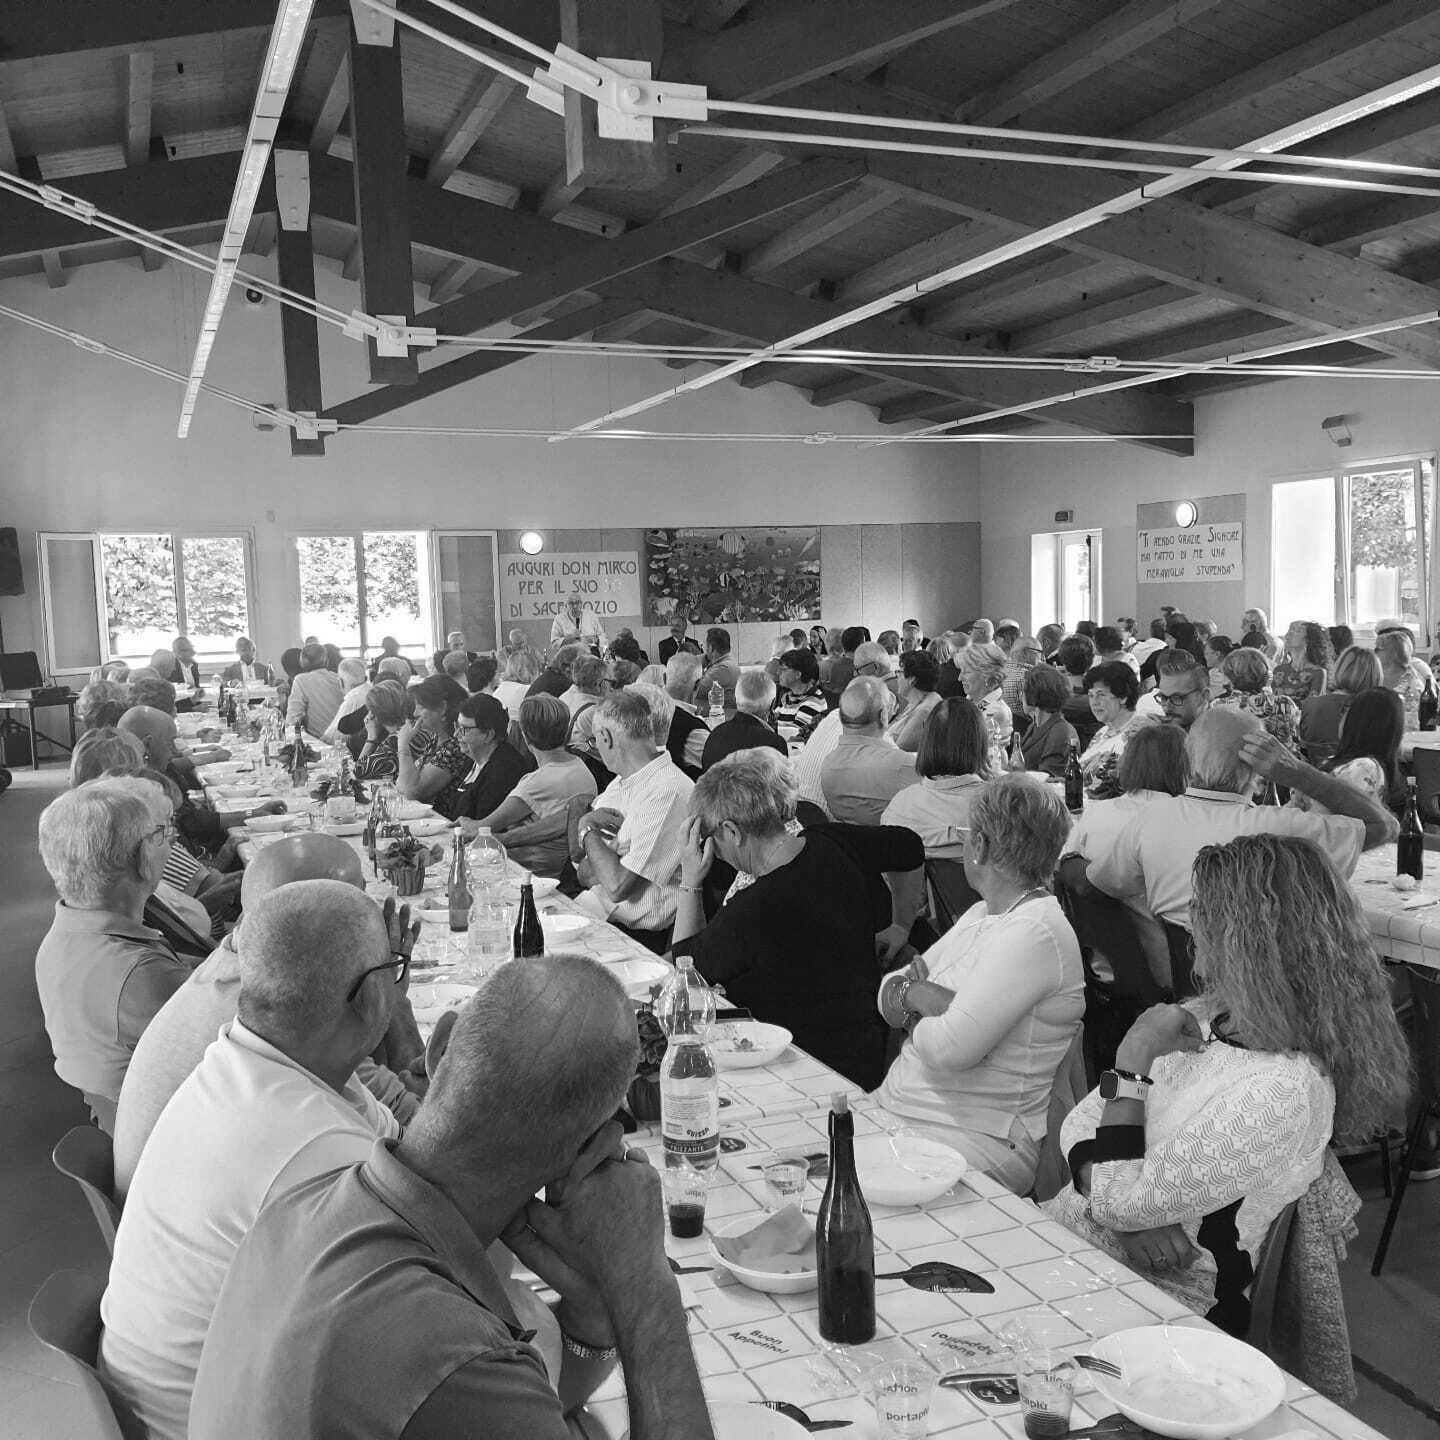
\includegraphics[width=\textwidth]{don-mirco-3}
\end{minipage}
\hfill
\begin{minipage}{0.47\textwidth}
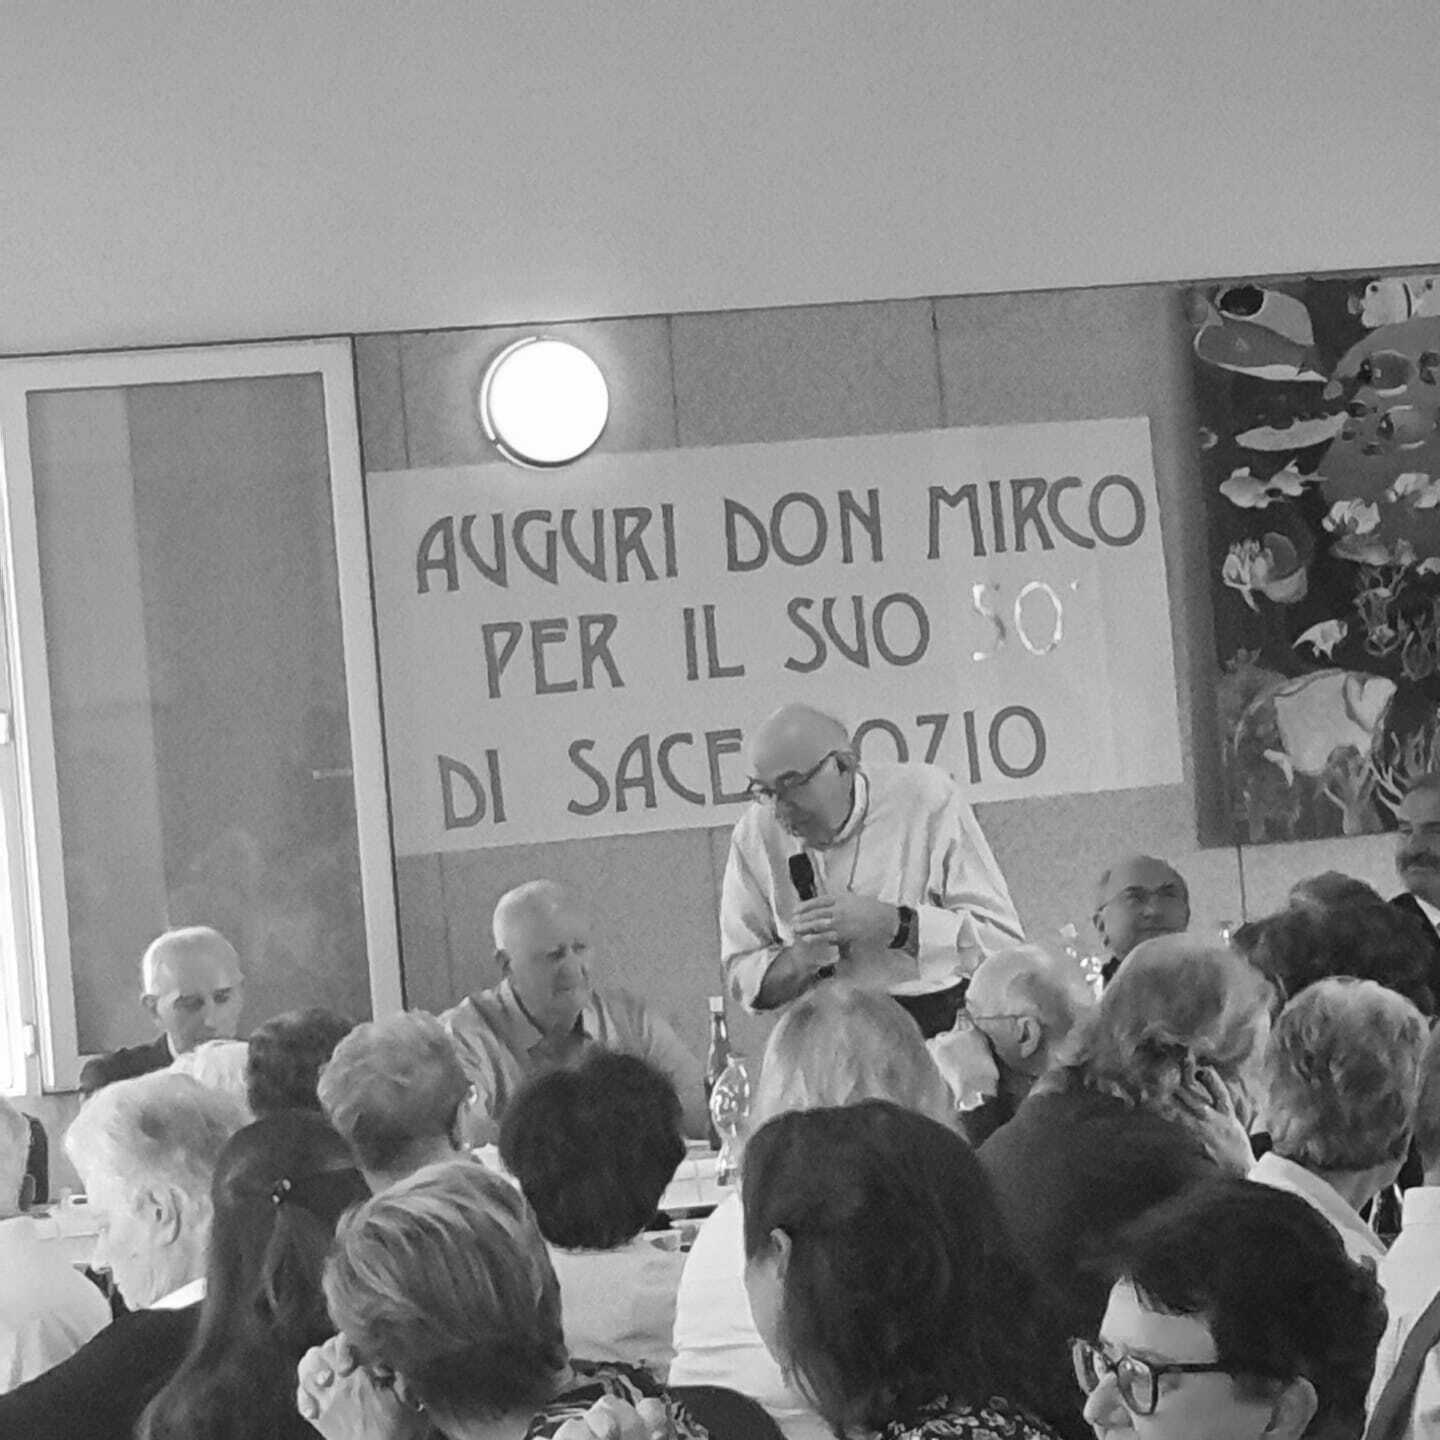
\includegraphics[width=\textwidth]{don-mirco-4}
\end{minipage}
\end{figure*}

È stata una bella domenica lo scorso 22 settembre perché la comunità ha voluto festeggiare il meraviglioso traguardo di Don Mirco sacerdote da cinquanta anni
\figurawrapdx{0.6\textwidth}{don-mirco-1}
(nominato il 21 settembre del 1974) e parroco a Maserada da ventiquattro (ingresso il 15 gennaio 2001).
La giornata ha avuto inizio con la S. Messa solenne delle 10.30 celebrata assieme ad altri sacerdoti amici e con tanti parenti che hanno voluto essere presenti affianco a Don Mirco in questa giornata solenne.

Don Mirco ha guidato spiritualmente tutti noi in questi anni e ha lasciato un segno indelebile nei nostri cuori. Gli siamo grati per l'amore che ci ha donato e per tutti i suoi insegnamenti e per questo motivo un grande numero di volontari ha voluto impegnarsi per organizzare al meglio la giornata. Il pranzo comunitario alla scuola comunale è stato l'evento centrale della giornata. Circa 160 fra parrocchiani, amici, parenti, sacerdoti e collaboratori pastorali hanno partecipato al pranzo.

\figuramedia{0.9\textwidth}{don-mirco-2}

Fra una portata e l'altra Don Mirco si è intrattenuto con i commensali coinvolto in simpatici discorsi, canti, barzellette, giochi e un'intervista che ha ripercorso alcuni momenti importanti del suo lungo sacerdozio. Hanno voluto raccontare aneddoti e condividere ricordi alcuni sacerdoti presenti, alcuni parenti e le autorità comunali. Al termine del pranzo c'è stato il fatidico taglio della torta corredato da applausi e fotografie.

\firma{Massimiliano G.}


